\section{Special Situation} %5.2
First, visualizations were performed using \sys{Variable Importance} function. According to Figure \ref{4.3.2-Variance-Importance}, it can be seen that ozone, rainfall, and temperature are the most important features. However, rainfall is not as closely related to climate change as temperature, so we chose ozone and temperature as two key factors.

\begin{figure}[htbp]
\centering
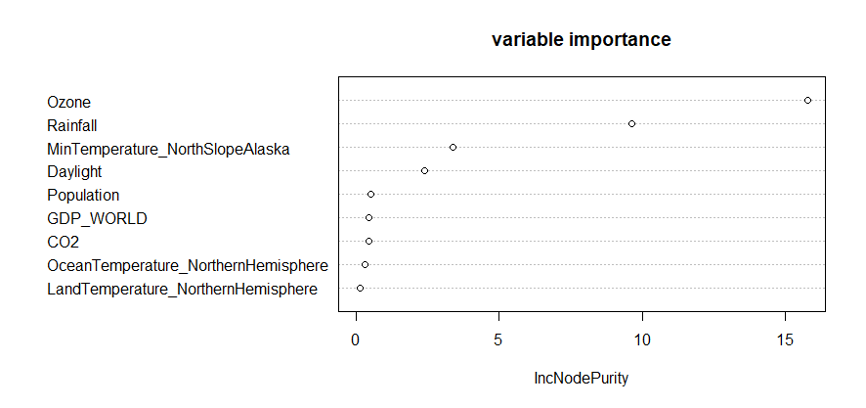
\includegraphics[width = 1.0\textwidth]{Figure/4.3.2-Variance-Importance.png}
\caption{Comparison of variance importance.}
\label{4.3.2-Variance-Importance}
\end{figure}

Linear Regression was applied on annul average ozone value only, a straight line was plotted and the ozone level decreased by 4.6\% in last 40 years. Based on the \sys{Normal Situation} data processing (Section \ref{sec:normal-predic}), the ozone level was predicted to decrease about 1.2\% in 10 years. For generating ozone data of \sys{Special Situation}, a ramp was applied on \sys{Normal Situation} data for simulating ozone variation in high level where it was decreased by 2.5\% in 10 years and low level where it was set no variation in 10 years).

\begin{figure}[htbp]
\centering
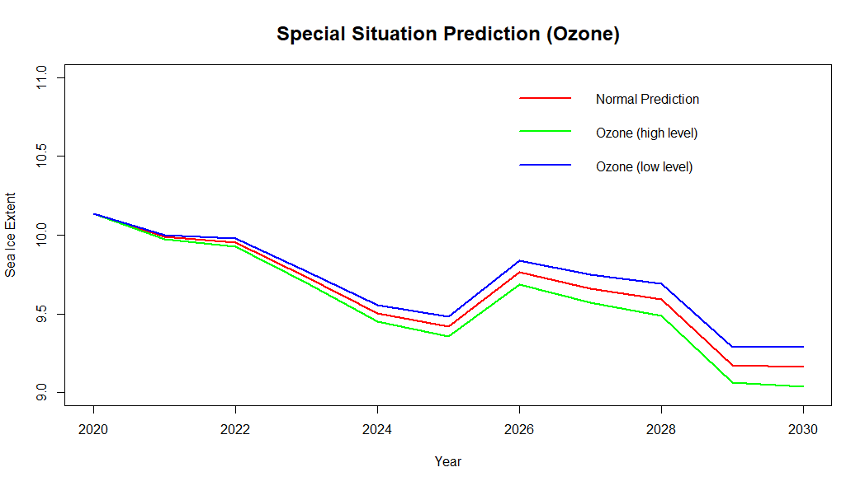
\includegraphics[width = 1.0\textwidth]{Figure/4.3.2-Emergency-Prediction-Ozone.png}
\caption{Special situation prediction based on different Ozone level.}
\label{4.3.2-Emergency-Prediction-Ozone}
\end{figure}

As Figure \ref{4.3.2-Emergency-Prediction-Ozone} shown, applying high level ozone, the predicted extent of Arctic sea ice was 0.92\% lower than applying Normal Situation, which was 9.414 $\text{Mkm}^2$. Moreover, applying low level ozone level, the predicted result was 0.87\% higher than that of \sys{Normal situation}. There was a negative correlation between ozone level and Arctic ice extent, which further confirmed the relationship shown in correlation matrix.

Similarly, applying the same method on \textit{MinTemperature}, in high level, normal situation and low level, the temperature was set to rise by 7,4,1 degree Celsius respectively.


\begin{figure}[htbp]
\centering
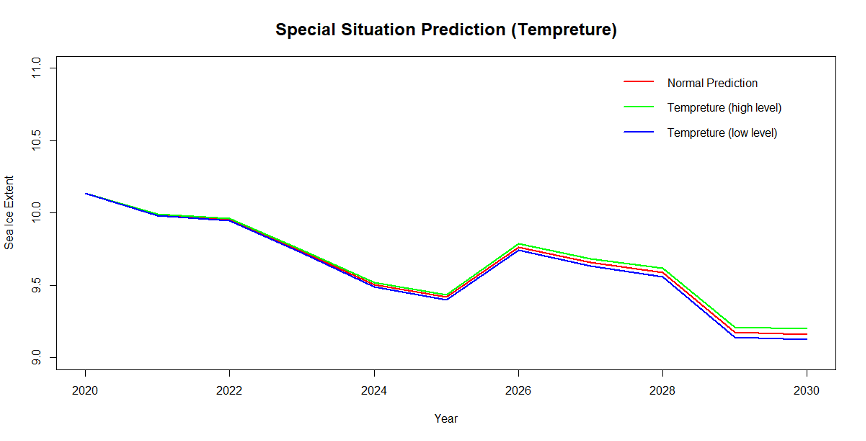
\includegraphics[width = 1.0\textwidth]{Figure/4.3.2-Emergency-Prediction-Temp.png}
\caption{Special situation prediction based on different minimum temperature level in North Slope Alaska.}
\label{4.3.2-Emergency-Prediction-Temp}
\end{figure}

According to the results above (Figure \ref{4.3.2-Emergency-Prediction-Temp}), applying high level temperature, the predicted extent of Arctic sea ice was 0.13\% higher than applying Normal Situation. While applying low level ozone level, the predicted result was 0.16\% lower than \sys{Normal situation}. It was found that the temperature is positively correlated with the Arctic sea ice extent from the correlation matrix. In addition, the influence of temperature change on the sea ice extent is not as sensitive as ozone, which also proved the feature importance of temperature is lower than ozone.